\chapter{Kapitelname}
\label{chap:abc}

section{Unterkapitel}
\label{sec:abc-uk}

\subsection{Unterunterkapitel}
\label{sec:abc-uk-uuk}



\textbf{Man} kann mit den labels im Text bezug nehmen mit \autoref{sec:abc-uk-uuk}. Wenn man zitieren m�chte, dann verwendet man am besten  \citep[vgl.][S.~1]{Petkovic}. Ich denke die Logik wird klar, wenn man es hier betrachtet. Anf�hrungszeichen \textit{im Flie�text} erfolgen mittels \dq Wort\dq\space manchmal ben�tigt man das space um ein Leerzeichen zu generieren.
\subsubsection{Fette �berschrift}
\label{sec:abc-uk-uuk-uuuk}

F�r Bilder k�nnt ihr folgendes copy pasten. Die Bilder, die ihr einf�gen m�chtet, sollten im Ordner fig eingef�gt werden. Hier sollte bei includegraphics der Name eingesetzt werden, caption steht f�r Bildunterschrift und das label muss individuell sein damit man darauf referenzieren kann. 

\begin{figure}[H]
	\centering
	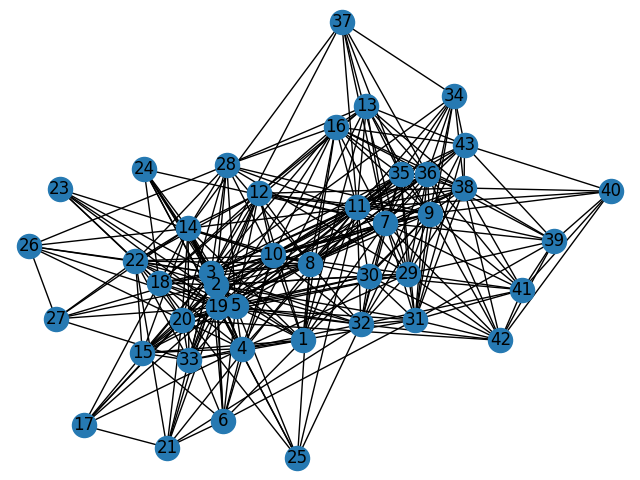
\includegraphics[width=10cm]{fig/beachego}
	\caption{Ego-Netzwerk des Datensatzes}
	\label{img:beachego}
\end{figure}

Bei mehreren Bildern nebeneinander k�nnt ihr folgendes verwenden: 

\begin{figure}[h]
	\centering
	\subfloat{
		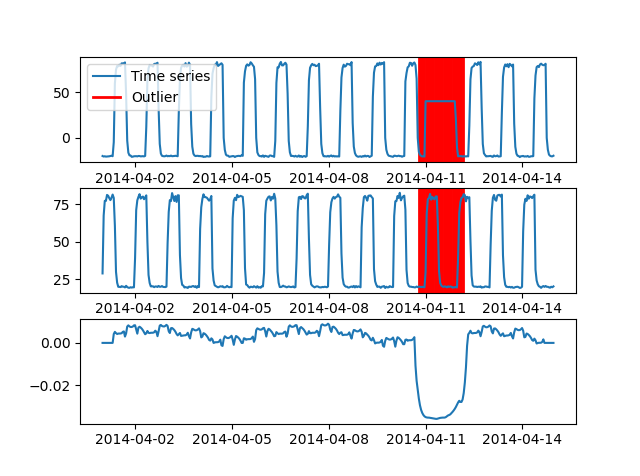
\includegraphics[width=0.5\textwidth]{fig/vardir1_1}}
	\subfloat{
		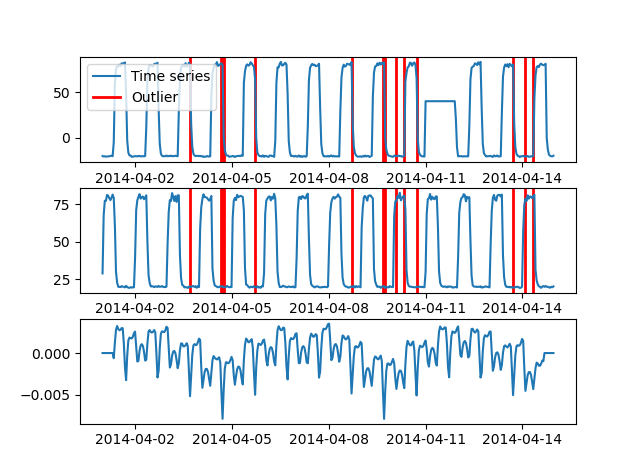
\includegraphics[width=0.5\textwidth]{fig/vardir1_2}}
	\qquad
	\subfloat{
		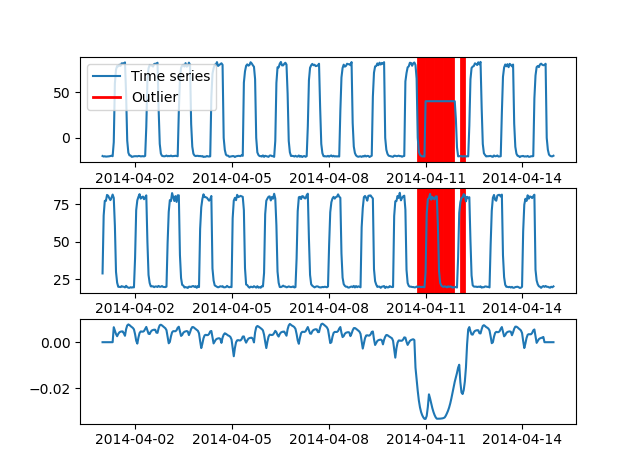
\includegraphics[width=0.5\textwidth]{fig/vardir1_3}}
	\subfloat{
		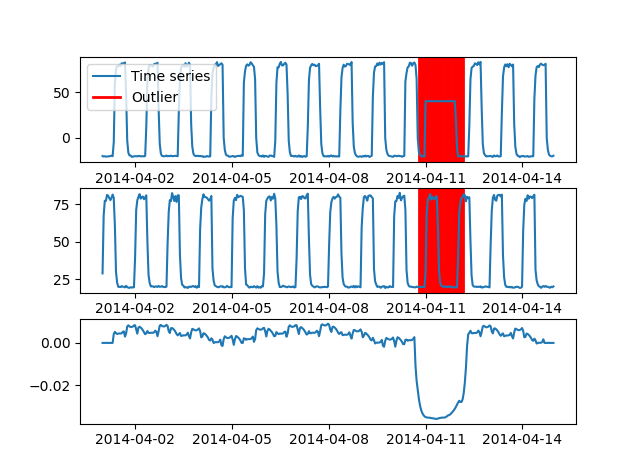
\includegraphics[width=0.5\textwidth]{fig/vardir1_4}}
	\caption{Im Uhrzeigersinn: an erster Variablen ausgerichtet (Variante 1), an zweiter Variablen ausgerichtet (Variante 2), nicht ausgerichtet (Variante 3) und an allen Variablen ausgerichtet (Variante 4).}
	\label{img:vardir1}
\end{figure}

Wenn ihr to dos vermerken wollt, nutzt hierf�r: 
\workTodo{hier ein to do einf�gen}


Wenn ihr etwas aufz�hlen wollt:

\begin{enumerate}
	\item Verschaffen eines �berblicks �ber die existierenden Algorithmen zur Erkennung von Ausrei�ern in Graphen
	\item Die Entwicklung eines Ausrei�er-Scores f�r die zugrundeliegenden Algorithmen
	\item Erste Anwendung der verwendeten Graphen-basierten Algorithmen auf Zeitreihen 
\end{enumerate}